\documentclass[a4paper, british]{article}

\usepackage[utf8]{inputenc}
\usepackage[T1]{fontenc}
\usepackage{babel}
% \usepackage[margin=2.5cm,a4paper]{geometry}
% \usepackage[skip=1em]{parskip}
\usepackage{lmodern} 
\usepackage{microtype}
% \usepackage{xcolor}
\usepackage{graphicx}
\graphicspath{ {./figures/} }
\usepackage{float}
% \usepackage{enumitem}
\usepackage{adjustbox} % rescale - useful for Dia exported TeX
\usepackage{tikz}
% \usepackage{pgfplots}
\usepackage{booktabs} %tables no vertical lines
% \usepackage{array}
% \usepackage{authblk}
% \usepackage{fancyhdr} %headers and footers
% \usepackage{titlesec}
% \usepackage{tcolorbox} % framed text boxes
% \usepackage{mathtools, amssymb, amsthm}
% \usepackage{gensymb}
\usepackage{chemformula} % chemical formulae
\usepackage{chemfig} % molecular figures
\usepackage{siunitx}
\usepackage{csquotes}
\usepackage[titletoc, title]{appendix}
% \usepackage{lettrine} % initials

\usepackage[
pdfauthor={Adam Menne},
pdftitle={Chemistry 254 - Practical 1},
pdfsubject={},
pdfkeywords={}]{hyperref}

\usepackage[noabbrev]{cleveref}

\usepackage[
backend=biber,
style=numeric,
sorting=none,
doi=true,
isbn=false
]{biblatex}
\addbibresource{citations.bib}

\setlength{\parskip}{1em}
\setlength{\parindent}{0em}
\linespread{1.3}

\title{Chemistry 254\\ Experiment 11\\ Spectrophotometrical determination of the \(pK_A\) of methyl red}
\date{Last editted on \today}
\author{Adam Menne\\ Stellenbosch University}

\begin{document}

\maketitle

\begin{abstract}
\noindent
In this practical the acid dissociation constant of methyl red was determined using spectrophotometry.
\end{abstract}

\tableofcontents

\newpage

\section{Introduction}

In this practical we determine the acid dissociation constant (\(pK_A\)) of the indicator methyl red using spectrophotometry.

First two calibration solutions were made, for both the ionised and non-ionised forms of methyl red. The absorbance was measured at 520 \(nm\) and 425 \(nm\) for the ionised and non-ionised forms respectively, at various concentrations. From this we are able to obtain a calibration curve by taking linear regressions, the slope of the regression line allowes for the calculation of the relative concentrations of the acid and base forms of methyl red present in our test solutions. From this we calculate \(pK_A\) values for each test solution, of which the \(pH\) was also measured.

We compare these \(pK_A\) values against one obtained by taking the linear regression of pH against \(log \left( \frac{[MR^-]}{[MRH]} \right)\). This use of the Henderson-Hasselbalch equation means, the intercept of our regression line will give the value of the \(pK_A\). Furthemore providing a more accurate value then simply taking the mean of the values for each test solution.


\section{Results}
\Cref{fig:MRH}, and \cref{fig:MR} show the absorbance for \(MRH\) and \(MR^-\) at 520 \(nm\)and 425 \(nm\) respectively, at various concentrations, with the regression line.

\Cref{fig:pH} shows pH against \(log \left( \frac{[MR^-]}{[MRH]} \right)\) for the test solutions, with regression line.

Our average \(pK_A\) value of 6.630 has a standard deviation of 0.354. The value calculated from the linear regression shown in \cref{fig:pH} is 5.903. 

\begin{figure}[h!]
    \centering
    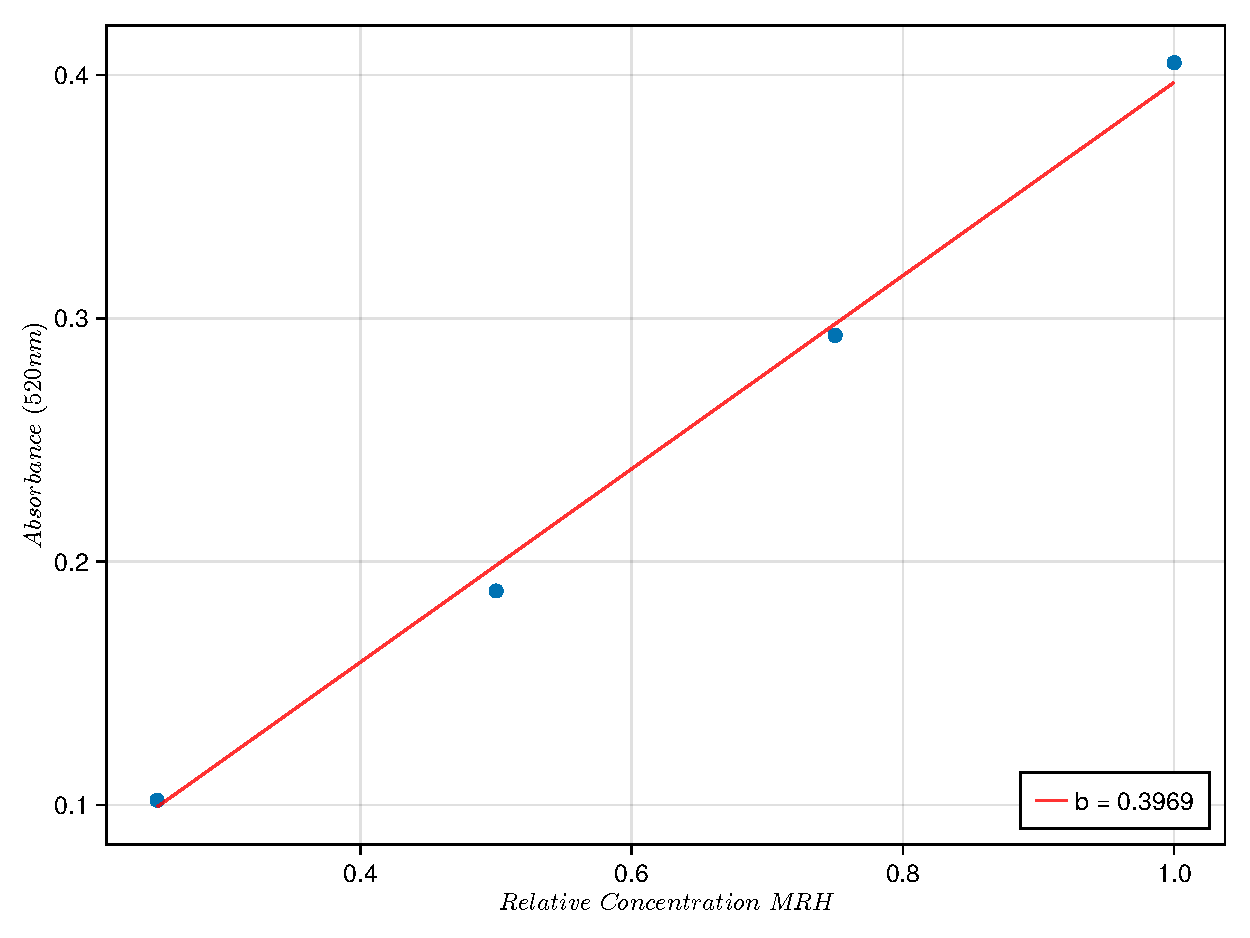
\includegraphics[width=0.75\textwidth]{figures/MRH}
    \caption{Absorbance at \(520\ nm\)}
    \label{fig:MRH}
\end{figure}

\begin{figure}[h!]
    \centering
    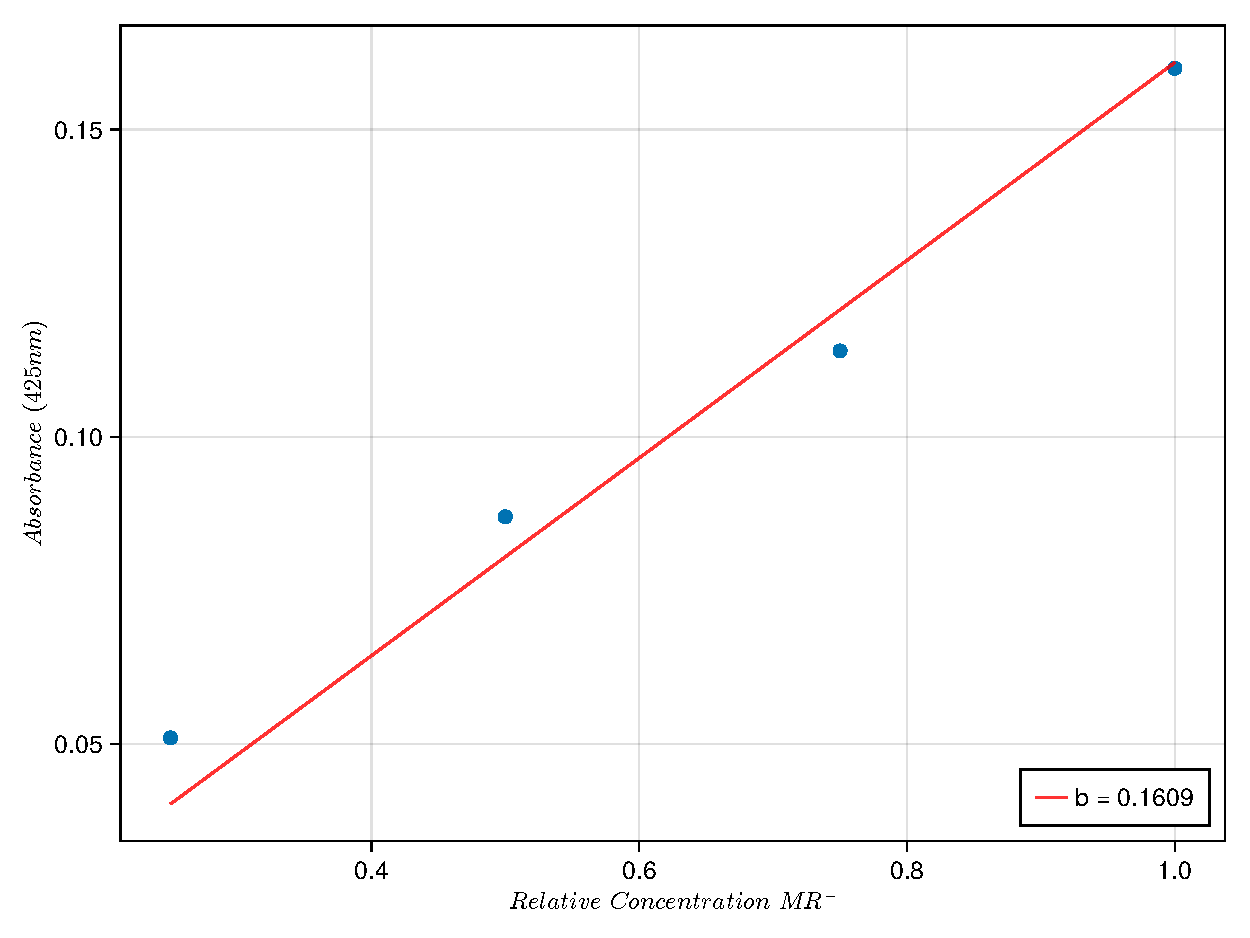
\includegraphics[width=0.75\textwidth]{figures/MR.pdf}
    \caption{Absorbance at \(425\ nm\)}
    \label{fig:MR}
\end{figure}

\begin{figure}[H]
    \centering
    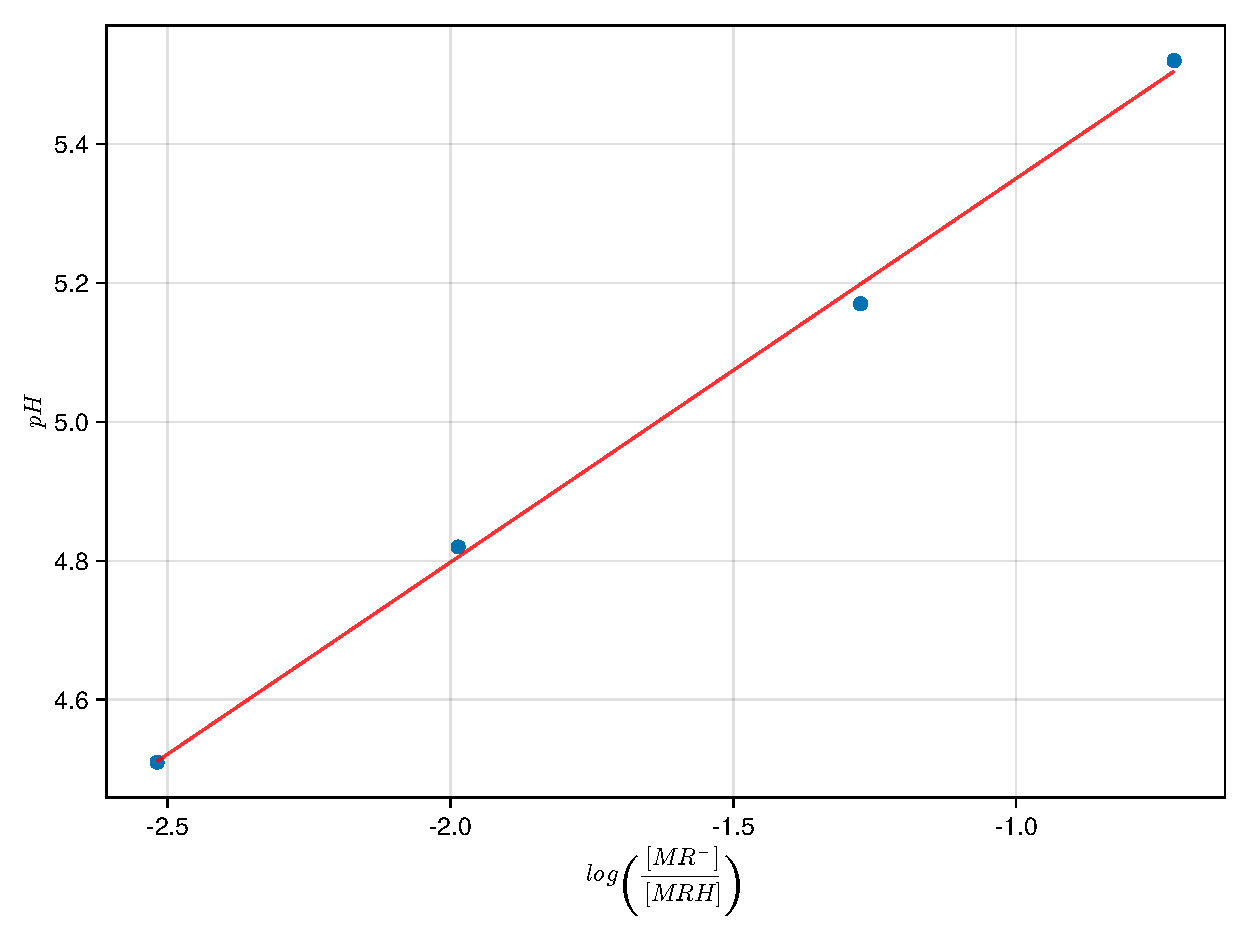
\includegraphics[width=0.75\textwidth]{figures/pH.pdf}
    \caption{pH over \(log \left( \frac{[MR^-]}{[MRH]} \right)\)}
    \label{fig:pH}
\end{figure}


A static export of the notebook containing all analysis and figures is availible at \url{https://adammenne.github.io/chemistry_254/practical_3/notebook.html}.\\ With full source code availble at \url{https://github.com/AdamMenne/chemistry_254/tree/master/practical_3}

\section{Discussion}

The value for \(pK_A\) detrmined by linear regression is notably lower than the mean value of the test solutions, and is closer to values referenced in the literature

However, both of these values deviate significantly from values referenced in the literature which range from 4.8 to 5.1. This is most likely due to the build up of various errors in the preparation of the calibration and test solutions. And possibly the influence of factors not taken into account by the procedure. 

\newpage

\begin{appendices}

\section{Questions}

\begin{enumerate}
    \item In the Henderson–Hasselbalch equation we take the log of the ratio of two concentrations, as such the exact values have no impact, only the value of this ratio.
    \item Probably, notably
    \item Most likely, however it is hard to say without knowing the actual concentration of the original methyl red solution. As, at high enough concentration, electrostatic interactions will begin to impact the absorbance, leading to values that deviate from what is expected according to the Beer-Lambert law.
\end{enumerate}

\newpage

\section{Flow Diagram}

\subsection*{A - Standard, acid, and base solutions}

\begin{enumerate}
    \item Prepare standard solution of 10 \(cm^3\) add 125\(cm^3\) 96\% \(C_2 H_5 OH\), make up with distilled water
    \item Prepare solution A with 50 \(cm^3\) of the standard solution and 50 \(cm^3\) 0.1 M \(HCl\), make up with water
    \item Prepare solution B with 50 \(cm^3\) of the standard solution and 100 \(cm^3\) 0.04 M \(CH_3 COONa\), make up with water
\end{enumerate}

\subsection*{B - Calibration solutions}

\begin{enumerate}
    \item Acid form
    \begin{enumerate}
        \item Dilute solution A to 0.75, 0.5, and 0.25 with 0.1 M \(HCl\) in 10 \(mL\) volumetric flasks.
        \item Measure absorbance at 520 \(nm\).
    \end{enumerate}
    \item Base form
    \begin{enumerate}
        \item Dilute solution B to 0.75, 0.5, and 0.25 with 0.04 M \(CH_3 COONa\) in 10 \(mL\) volumetric flasks.
        \item Measure absorbance at 425 \(nm\).
    \end{enumerate}
\end{enumerate}

\subsection*{C - Test solutions}

\begin{enumerate}
    \item Prepare test solutions in 100 \(mL\) volumetric flasks according to the table at the bottom of page 54 of the practical guide.
    \item Measure absorbance at 520 \(nm\) and 425 \(nm\) of each solution.
    \item Measure \(pH\) of each solution.
\end{enumerate}

\newpage

\section{MSDS}

\subsection*{Methyl red}

\begin{itemize}
    \item Health hazard, environmental hazard
    \item[-] suspected of being carcinogenic
    \item[-] if exposed, seek medical advice
    \item[-] avoid release to the environment
\end{itemize}

\subsection*{Hydrochloric acid}

\begin{itemize}
    \item Harmful, corrisive
    \item[-] may cause skin burns, eye damage and respiratory irritation, do not inhale
    \item[-] if in contact with skin or eyes wash for several minutes  
\end{itemize}

\subsection*{Sodium acetate}

\begin{itemize}
    \item Low concern
\end{itemize}
    
\end{appendices}

\end{document}